\documentclass{article}
\usepackage[utf8]{inputenc}
\usepackage[english, russian]{babel}
\usepackage{graphicx}
\graphicspath{ {./graphics/} }
\usepackage[a4paper, total={6in, 8in}]{geometry}
\pagestyle{empty} %
\usepackage[pageanchor]{hyperref}
\usepackage{enumitem}
\usepackage{listings}
\usepackage{amssymb}
\usepackage{amsmath}
\usepackage{indentfirst}

\begin{document}
  \begin{titlepage}
    \begin{center}
      Санкт-Петербургский политехнический университет \\Петра Великого
    \end{center}

    \begin{center}
      Физико-механический институт
    \end{center}

    \begin{center}
      Высшая школа прикладной математики и вычислительной\\ физики
    \end{center}

    \vspace{8em}

    \begin{center}
      \textbf{Отчет по лабораторной работе №1}\\
      \textbf{“Интервальный анализ”}
    \end{center}

    \vspace{\fill}

    \begin{flushright}
      \noindentВыполнили студент группы 5030102/10201:
      \hfill
      Скворцов Владимир Сергеевич \\
    \end{flushright}
    Преподаватель: \hfill Баженов Александр Николаевич

    \vspace{12em}

    \begin{center}
      Санкт-Петербург\\
      2024
    \end{center}
  \end{titlepage}

  \tableofcontents

  \newpage

  \section{Постановка задачи}

  Дана ИСЛАУ

  \[
    Ax = b, \ x = (x_1, x_2)
  \]

  с матрицей

  \[
    \text{mid} A = \begin{pmatrix}
      a_{11} & a_{12} \\
      a_{21} & a_{22}
    \end{pmatrix}
  \].

  Пусть матрица радиусов для \( A \) имеет вид

  \[
    \text{rad} A = \alpha \begin{pmatrix}
      1 & 1 \\
      1 & 1
    \end{pmatrix}
  \].

  Необходимо:

  \begin{itemize}
    \item Найти диапазон значений \( \alpha \), при которых
      \( 0 \in \det A \);
    \item Для минимального значения радиуса матричных элементов
      \( \min \alpha \) найти точечную матрицу \( A' \):
      \[
        \det A' = 0.
      \]
  \end{itemize}

  \section{Необходимая теория}

  Интервалом вещественной оси \( [a, b] \), называется множество всех
  чисел, расположенных между заданными числами \( a \) и \( b \) включая
  их самих, т.е.

  \begin{equation}
    [a, b] \stackrel{\text{def}}{=}
    \left \{ x \in \mathbb{R} \mid a \leqslant x \leqslant b \right \}.
  \end{equation}

  При этом \( a \) и \( b \) называются концами интервала.

  \subsection{Интервальная арифметика}

  Развернутые формулы основных арифметических операций для интервалов:

  \begin{enumerate}
  \item \textbf{Сложение}
    \begin{equation}
      \mathbf{x} + \mathbf{y} = \left [ \underline{\mathbf{x}} + \underline{\mathbf{y}}, \ \overline{\mathbf{x}} + \overline{\mathbf{y}} \right ],
    \end{equation}
  \item \textbf{Вычитание}
    \begin{equation}
      \mathbf{x} - \mathbf{y} = \left [ \underline{\mathbf{x}} - \overline{\mathbf{y}}, \ \overline{\mathbf{x}} - \underline{\mathbf{y}} \right ],
    \end{equation}
  \item \textbf{Умножение}
    \begin{equation}
      \mathbf{x} \cdot \mathbf{y} = \left [
        \min \{
          \underline{\mathbf{x}} \ \underline{\mathbf{y}},
          \underline{\mathbf{x}} \ \overline{\mathbf{y}},
          \overline{\mathbf{x}} \ \underline{\mathbf{y}},
          \overline{\mathbf{x}} \ \overline{\mathbf{y}}
        \}, \
        \max \{
          \underline{\mathbf{x}} \ \underline{\mathbf{y}},
          \underline{\mathbf{x}} \ \overline{\mathbf{y}},
          \overline{\mathbf{x}} \ \underline{\mathbf{y}},
          \overline{\mathbf{x}} \ \overline{\mathbf{y}}
        \}
      \right ],
    \end{equation}
  \item \textbf{Деление}
    \begin{equation}
      \mathbf{x} / \mathbf{y} = \mathbf{x} \cdot \left [ 1 / \overline{\mathbf{y}}, \ 1 / \underline{\mathbf{y}} \right ], \ 0 \notin \mathbf{y}.
    \end{equation}
  \end{enumerate}

  \clearpage

  Формулы для характеристик интервала:

  \begin{enumerate}
  \item \textbf{Средняя точка}
    \begin{equation}
      \text{mid} \ \mathbf{x} = \frac{1}{2} (\underline{\mathbf{x}} + \overline{\mathbf{x}}).
    \end{equation}
  \item \textbf{Ширина}
    \begin{equation}
      \text{wid} \ \mathbf{x} = \overline{\mathbf{x}} - \underline{\mathbf{x}}.
    \end{equation}
  \item \textbf{Радиус}
    \begin{equation}
      \text{rad} \ \mathbf{x} = \frac{1}{2} (\overline{\mathbf{x}} - \underline{\mathbf{x}}).
    \end{equation}
  \end{enumerate}

  \section{Реализаця}

  Лабораторная работа выполнена на языке программирования Python. В ходе
  работы были также использованы библиотеки \verb!numpy! и
  \verb!matplotlib!.

  Ссылка на GitHub репозиторий:
  \href{https://github.com/vladimir-skvortsov/spbstu-interval-anylysis}{https://github.com/vladimir-skvortsov/spbstu-interval-anylysis}

  \subsection{Алгоритм поиска минимального \( \alpha \)}

  В ходе выполнения работы было найдено минимальное значение параметра
  \( \alpha \), при котором определитель интервальной матрицы \( A \)
  включает ноль (\( 0 \in \det A \)).

  Для нахождения минимального значения \(\alpha\) использовался
  итеративный метод с переменным шагом:

  \begin{enumerate}
    \item \textbf{Начальный этап}:
      \begin{itemize}
        \item Стартовое значение: \( k = 0 \), \(\alpha_0 = e^0 = 1\).
        \item На каждой итерации значение \( \alpha_k \) увеличивается по формуле:
          \[ k \to k + 1, \ \alpha_{0} = e^{k}. \]
        \item Процесс продолжается, пока \( 0 \notin \det A \).
      \end{itemize}

    \item \textbf{Уточнение значения}:
      \begin{itemize}
        \item Задаем точность \( \varepsilon > 0 \).
        \item Принимаем \( a_0 = 0 \) и \( b_0 = \alpha_0 \).
        \item Находим \( \alpha_{k+1} = \frac{a_k + b_k}{2} \).
        \item Если \( 0 \in \det A \), то \( b_{k+1} = \alpha_{k+1} \),
          иначе \( a_{k+1} = \alpha_{k+1} \).
        \item Процесс продолжается, пока \( b - a > \varepsilon \).
        \item Если \( b - a \leqslant \varepsilon \), возвращаем
          \( \frac{a_k + b_k}{2} \).
      \end{itemize}
  \end{enumerate}

  \clearpage

  \subsection{Результаты вычислений}

  \begin{table}[htbp!]
    \centering
    \renewcommand{\arraystretch}{1.2}
    \begin{tabular}{|c|c|c|}
      \hline
      k & \( \alpha_k \) & \( \det A_k \) \\
      \hline
      0 & 0.50000 & \([-1.90000, 2.10000]\) \\
      \hline
      1 & 0.25000 & \([-0.90000, 1.10000]\) \\
      \hline
      2 & 0.12500 & \([-0.40000, 0.60000]\) \\
      \hline
      3 & 0.06250 & \([-0.15000, 0.35000]\) \\
      \hline
      4 & 0.03125 & \([-0.02500, 0.22500]\) \\

      \hline
      \vdots & \vdots & \vdots \\
      \hline

      14 & 0.02499 & \([0.00002, 0.19998]\) \\
      \hline
      15 & 0.02500 & \([-0.00004, 0.20004]\) \\
      \hline
      16 & 0.02500 & \([-0.00000, 0.20000]\) \\
      \hline
    \end{tabular}
    \caption{Итерационный процесс при \( \varepsilon = 10^{-5} \)}
    \label{table:iterations}
  \end{table}

  Итерационный процесс представлен в таблице~\ref{table:iterations}.
  Из таблицы видно, что на 16-й итерации было найдено значение \( \alpha \)
  при заданной точности:

  \[ \alpha_{min} = 0.025 \]

  \subsection{Итоговые результаты}

  Минимальное значение параметра регуляризации:

  \[ \alpha_{min} = 0.025 \]

  При этом интервальная матрица \(A\) имеет следующий вид:

  \[
    A = \begin{bmatrix}
      [1.025,\ 1.075] & [0.925,\ 0.975] \\
      [0.975,\ 1.025] & [0.975,\ 1.025]
    \end{bmatrix}
  \]

  Определитель данной матрицы составляет:

  \[ det(A) = [0.0,\ 0.2] \]

  Диапазон значений \( \alpha \), при котором определитель интервальной
  матрицы \( A \) включает ноль, составляет:

  \[ \alpha \in [0.025,\ +\infty) \]

  \subsection{Нахождение точечной матрицы \( A' \)}

  Для найденного минимального значения \( \alpha_{min} \) была определена
  точечная матрица \( A' \), принадлежащая интервальной матрице \( A \),
  такая, что \( \det A' = 0 \).

  Точечная матрица \( A' \) имеет вид:

  \[
    A' = \begin{bmatrix}
      1.025 & 0.975 \\
      1.025 & 0.975
    \end{bmatrix}
  \]

  Эта матрица является вырожденной, так как её строки линейно зависимы, и
  определитель равен нулю.

  \subsection{Скорость сходимости}

  \begin{figure}[htbp!]
		\begin{center}
			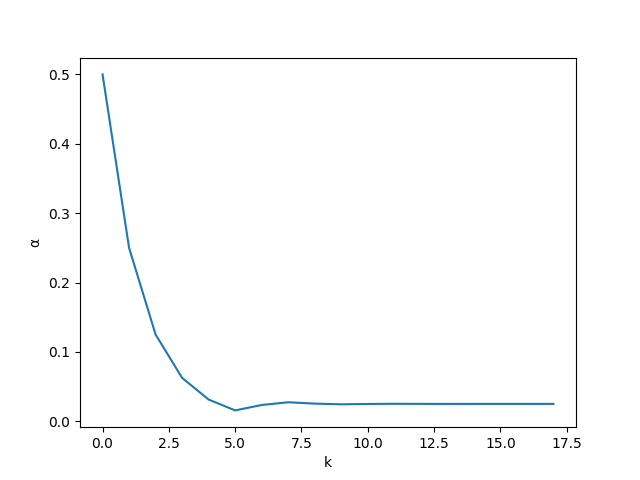
\includegraphics[width = 0.6\textwidth]{values}
			\caption{Зависимость значения \( \alpha \) от номера итерации \( k \)}
      \label{figure:values}
		\end{center}
	\end{figure}

  \begin{figure}[htbp!]
		\begin{center}
			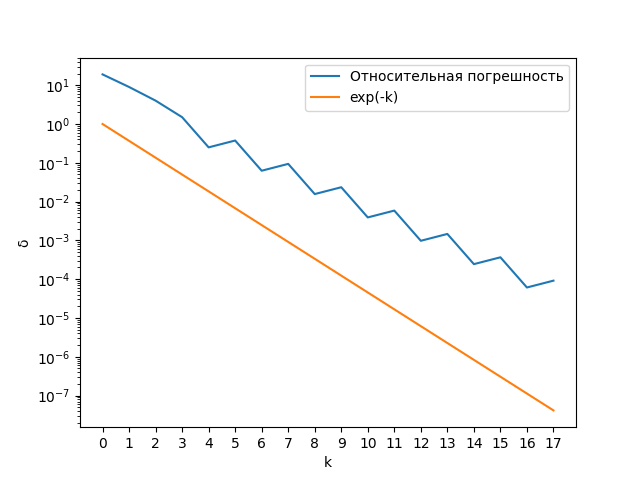
\includegraphics[width = 0.6\textwidth]{relative-errors}
			\caption{Относительная погрешность \( \delta \) от номера
        итерации \( k \)}
      \label{figure:relative-errors}
		\end{center}
	\end{figure}

  Из графика~\ref{figure:relative-errors} следует, что относительная
  погрешность уменьшается с темпом, близким к \( \exp(-k) \).

  \clearpage

  \section{Обсуждение}

  \begin{enumerate}
    \item \textbf{Физическая интерпретация} \\
      Матрица \( A' \) представляет собой матрицу, формируемую при
      минимальном значении радиуса матричных элементов \( \delta \). Это
      минимальное значение радиуса соответствует моменту, когда матрица
      \( A \) теряет свою обратимость, и \( \det A' = 0 \). Следовательно,
      система уравнений становится вырожденной, что означает наличие
      бесконечного множества решений. В физическом смысле это указывает на
      то, что данные, полученные с двух ракурсов, недостаточны для точной
      реконструкции объекта, поскольку отсутствует информация для
      однозначного решения.
    \item \textbf{Чувствительность при минимальном радиусе} \\
      При минимальном радиусе матричных элементов формируется точечная
      матрица \( A' \), которая представляет собой границу множества
      возможных матриц \( A \), описывающих интервал неопределенности.
      Система становится чувствительной к незначительным возмущениям в
      данных. Любое изменение исходных данных может существенно повлиять
      на результат реконструкции, что усложняет задачу томографии в
      условиях реальных данных с шумами.
    \item \textbf{Практические соображения} \\
      В практической томографии часто используется большее количество
      ракурсов, чем два, для улучшения условий задачи и предотвращения
      ситуации, когда \( detA' = 0 \). В задачах с ограниченным числом
      ракурсов проблема вырожденности матрицы возникает часто, поэтому
      такие задачи требуют применения специальных методов, учитывающих
      неоднозначность.
  \end{enumerate}

  \section{Выводы}

  В ходе лабораторной работы была построена интервальная матрица \(A\)
  размером \(2 \times 2\) следующего вида:

  \[
    A = \begin{bmatrix}
      [1.05 - \alpha, 1.05 + \alpha] & [0.95 - \alpha, 0.95 + \alpha] \\
      [1 - \alpha, 1 + \alpha] & [1 - \alpha, 1 + \alpha]
    \end{bmatrix}
  \]

  Для данной матрицы был вычислен диапазон значений \(\alpha\), при которых
  определитель интервальной матрицы включает ноль, что соответствует
  состоянию вырождения матрицы. Минимальное значение \(\alpha = 0.025\)
  было установлено с использованием итерационного алгоритма с переменным
  шагом.

  При этом было установлено, что при значении \( \alpha = 0.025 \)
  интервальный определитель матрицы принимает значения в интервале
  \( [0.0, 0.2] \), что включает ноль. Следовательно, это значение
  \( \alpha \) является минимальным, при котором матрица \( A \) становится
  вырожденной.

  Для минимального значения \( \alpha \) была найдена точечная матрица
  \(A'\), принадлежащая интервальной матрице \( A \), такая, что:

  \[
    A' = \begin{bmatrix}
      1.025 & 0.975 \\
      1.025 & 0.975
    \end{bmatrix}
  \]

  Эта матрица является вырожденной, поскольку её строки линейно зависимы,
  и её определитель равен нулю.

  В общем случае, если матрица \( A \) представляет собой матрицу линейной
  регрессии, она может иметь размерность \(2 \times N\) (где \(N \geq 2\)) и
  не быть квадратной. В таких случаях для анализа необходимо рассматривать
  всевозможные квадратные подматрицы и для каждой подбирать своё значение
  \( \alpha \), при котором эти матрицы будут неособенными
  (невырожденными). Затем, пересечение всех найденных матриц позволяет
  получить итоговую регуляризованную матрицу, которая удовлетворяет
  условиям задачи и может быть использована для дальнейшего анализа или
  вычислений.
\end{document}
